% Identity Plot
% Variations of the Bland Altman Plot
% Survival Plot (Luiz et al)
% Bartko's Ellipse
% Mountain Plot

\documentclass[Chap2main.tex]{subfiles}
\begin{document}
	
	
	

\subsection{The Identity plot} This is a simple regression based approach. It gives the analyst a cursory examination of how well the measurement methods agree. In the case of good agreement, the covariates of the plot accord closely with the $X=Y$ line.

\subsection{Variations of the BA plot}

In light of some potential pitfalls associated with the conventional BA plot, a series of alternative formulations for the Bland-Altman plot have been proposed.

\newpage
\subsection{Bartko's Ellipse}
\citet{Bartko} offers a graphical complement to the Bland-Altman
plot, in the form of a bivariate confidence ellipse.
\citet{AltmanEllipse} provides the relevant calculations.

\begin{figure}[h!]
	% Requires \usepackage{graphicx}
	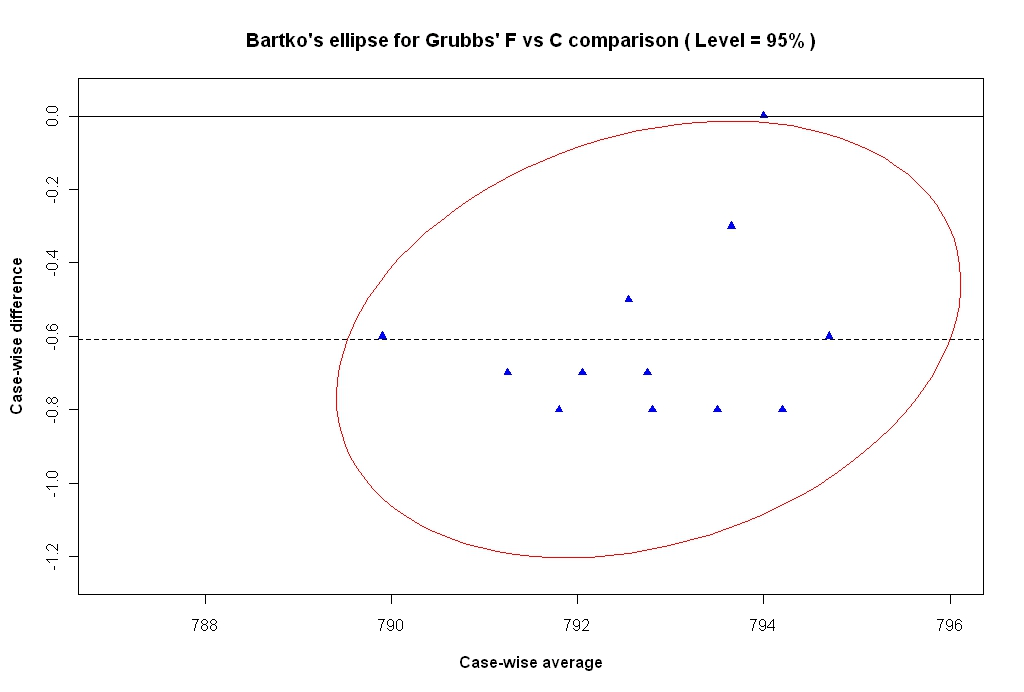
\includegraphics[width=130mm]{GrubbsBartko.jpeg}
	\caption{Bartko's Ellipse For Grubbs Data}\label{GrubbsBartko}
\end{figure}



\section{Survival Agreement Plot (Luiz et al)}
This approach is put forward by \textit{Luiz}. It seeks to extend the agreement evaluation through a graphic approach using step functions' capable of expressing the degree of agreement (or disagreement) as a function of several limits of tolerance.

\begin{itemize}
\item It expresses agreement or disagreement as a function of several
limits of tolerance.
\item Y axis represents the proportion of discordant cases.
\item X axis represents the observed differences.
\end{itemize}

\section{Eksborg's Plot}
\textit{Eksborg} proposes a plot of the relative values found by the two
Methods being compared (Method 1/Method 2) vs the mean of the Method
values.

This approach was discussed as an alternative to the BA approach by 
%%%%%%%%%%%%%%%%%%%%%%%%%%%%%%%%%%%%%%%%%%%%%%%%%%%%%%%%%%%%%%%%%%%%%%%%%
\newpage
\section{Bartko's Ellipse}
As an enhancement on the Bland Altman Plot, \textit{bartko} has
expounded a confidence ellipse for the covariates. \textit{bartko} proposes
a bivariate confidence ellipse as a boundary for dispersion. The stated purpose is to 'amplify dispersion', which presumably is for  the purposes of outlier detection.The orientation of the the ellipse is key to interpreting the results.
\begin{itemize}
 \item The Minor Axis is related to the Variance between-subjects
 \item The Major Axis is related to the Error Mean Square.
\end{itemize}
The ellipse illustrates the size of both relative to each
other. Furthermore, the ellipse provides a visual aid to determining the relationship
between the variance of the means $Var(a_{i})$ and the variance of the differences $Var(d_{i})$.
\begin{itemize}
 \item If $Var(a_{i})$ is greater than $Var(d_{i})$, the orientation of the ellipse is horizontal.
 \item If $Var(a_{i})$ is less than $Var(d_{i})$, the orientation of the ellipse is vertical.
\end{itemize}
The more horizontal the ellipse, the greater the ICC.

\newpage



%----------------------------------------------------------------%
\section{Dewitte et al }
Bland ALtman recommend the logarithmic y scale
others prefer the  precent y scale.
generally there is not much difference(except when the data extends over several orders of magnitude)
percent method is recommends becuase the numbers can be read directly from the plot without the need for back transfromation.

\begin{verbatim}
absolute - small range
percentage - medium range
log scale - large range
\end{verbatim}
we observe increasing use of the bland altman plot over the years, from 8% in 1995 to 14% in 1996 and 31%to36% in more recent years.

% MCS Mountain Plot Notebook
\newpage
\section{Mountain Plot} Krouwer and Monti have proposed a folded empirical cumulative distribution plot, otherwise known as a Mountain plot.

They argue that it is suitable for detecting large, infrequent errors. This is a non-parametric method that can be used as a complement with the Bland Altman plot.  Mountain plots are created by computing a percentile
for each ranked difference between a new method and a reference method. (Folded plots are so called because of the following transformation is performed for all percentiles above 50: percentile = 100 - percentile.) These percentiles are then plotted against the differences between the two methods.

Krouwer and Monti argue that the mountain plot offers some following advantages. It is easier to find the central $95\%$ of the data, even when the data are not normally distributed. Also, comparison on different distributions can be performed with ease.

\emph{
	A mountain plot (or "folded empirical cumulative distribution plot") is created by computing a percentile for each ranked difference between a new method and a reference method. To get a folded plot, the following transformation is performed for all percentiles above 50: percentile = 100 - percentile. These percentiles are then plotted against the differences between the two methods (Krouwer and Monti, 1995).}

\emph{
	The mountain plot is a useful complementary plot to the Bland and Altman plot. In particular, the mountain plot offers the following advantages:}
\emph{
	It is easier to find the central $95\%$ of the data, even when the data are not Normally distributed.
	Different distributions can be compared more easily.
}
\newpage
%------------------------------------------------------------------------------%
% http://peer.ccsd.cnrs.fr/docs/00/75/39/50/PDF/PEER_stage2_10.1016%252Fj.spl.2011.03.014.pdf
The folded cumulative distribution function for a random variable can be easily obtained by folding down the upper half of the cumulative distribution
function (CDF). It is a simple graphical method for summarising distributions, and has been used for the evaluation of laboratory assays, clinical trials
and quality control (Monti, 1995; Krouwer and Monti, 1995).

%------------------------------------------------------------------------------%

% http://www.ncbi.nlm.nih.gov/pubmed/8547437

A mountain plot (or ``folded empirical cumulative distribution plot") is created by computing a percentile for each ranked difference between a new method and a reference method. 

To get a folded plot, the following transformation is performed for all percentiles above 50: 
percentile = 100 – percentile. These percentiles are then plotted against the differences between 
the two methods (Krouwer \& Monti, 1995). The calculations and plots are simple enough to perform in a spreadsheet. 

The mountain plot is a useful complementary plot to the Bland \& Altman plot. 
In particular, the mountain plot offers the following advantages:
%------------------------------------------------------------------------------%
\begin{itemize}
	\item It is easier to find the central 95\% of the data, even when the data are not Normally distributed.
	\item Different distributions can be compared more easily.
	\item Unlike a histogram, the plot shape is not a function of the intervals. 
	%\item
	%\item
\end{itemize}

%------------------------------------------------------------------------------%

Compared with the Bland-Altman difference plot, the folded CDF stresses more the median and tails of the difference. 
If the two assays are ‘unbiased’ 98 with each other (Krouwer and Monti, 1995), the median would be close to zero. 
%If the variability between the two assays is large, the width near the 100 bottom of the folded CDF would be large, analogously to a confidence interval.

%------------------------------------------------------------------------------%
%Advantages 
% 1. It is easier to find the central 95\% of the data. 
% 2. It is easier to estimate percentile for large differences (e.g., percentiles greater than 95\%). 
% 3. Unlike a histogram, the plot shape is not a function of the intervals. 
% 4. Comparing different distributions is easier. 
% 5. The plot is easier to interpret than a standard empirical cumulative distribution plot. 

%------------------------------------------------------------------------------%

Bland-Altman and mountain plots each provide complementary perspectives on the data, and the authors recommend both plots.
%------------------------------------------------------------------------------%

\subsection{Survival Plots}

\begin{itemize}
	%----------------------------%
	% 1. **Background and Objective:** 
	
	\item Survival–agreement plots have been suggested as a new graphical approach to assess agreement in
	quantitative variables. We propose that survival analytical techniques can complement this method, providing a new analytical insight
	for agreement.
	
	%----------------------------%
	% 2. **Methods:** 
	
	\item Two survival–agreement plots are used to detect the bias between to measurements of the same variable. The presence of
	bias is tested with log-rank test, and its magnitude with Cox regression.
	%----------------------------%
	% 3. **Results:** 
	
	\item An example on C-reactive protein determinations shows how survival analytical methods would be interpreted in the context
	of assessing agreement.
	
	%----------------------------%
	% 4. **Conclusion:** 
	\item Log-rank test, Cox regression, or other analytical methods could be used to assess agreement in quantitative variables;
	correct interpretations require good clinical sense
	
\end{itemize}
%---------------------------------------------------------%


\bibliography{DB-txfrbib}
\end{document}
